\documentclass[10pt,twocolumn]{article}
\usepackage[margin=0.56in,top=0.60in,bottom=0.60in]{geometry}
\usepackage{amsmath,amssymb,amsthm}
\usepackage{booktabs}
\usepackage{graphicx}
\usepackage{microtype}
\usepackage[hidelinks]{hyperref}
\usepackage{xurl}

\raggedbottom
\setlength{\columnsep}{0.20in}
\setlength{\parskip}{1.5pt}
\setlength{\textfloatsep}{7pt plus 2pt minus 2pt}
\setlength{\dbltextfloatsep}{8pt plus 2pt minus 2pt}

\title{\vspace{-1.2em}\textbf{Exact Rational and Constructive Lean~4 Certificates for Triangles Without Pentagons, Induced $C_4$--$C_5$ Extremal Graphs, and 3-Uniform Berge-Cycle Hypergraphs}\vspace{-0.4em}}
\author{Lluis Eriksson\\
\small Independent Researcher (\nolinkurl{https://github.com/lluiseriksson})\\
\small Companion Preprint to Cui--Gy\H{o}ri--Zhang--Zhu (\texttt{arXiv:2611.33685v1}) --- Unrefereed Formal-Verification Artifact\vspace{-0.6em}}
\date{November 26, 2026}

\begin{document}
\maketitle

\begin{abstract}
\noindent Cui, Gy\H{o}ri, Zhang, and Zhu (\texttt{arXiv:2611.33685v1}, Nov.~2026) resolve the nineteen-year-old Bollob\'as--Gy\H{o}ri conjecture, proving $\mathrm{ex}(n, K_3, C_5) = (\tfrac{1}{3\sqrt{3}} + o(1))n^{3/2}$, together with the sharp induced-$C_4$--$C_5$ Tur\'an asymptotic $\mathrm{ex}(n,\{\mathrm{ind}\text{-}C_4, C_5\}) = \tfrac{2}{3\sqrt{3}}(1+o(1))n^{3/2}$ and the 3-uniform Berge-cycle conjecture $\mathrm{ex}_3(n,\{BC_3,BC_4,BC_5\}) = \tfrac{1+o(1)}{3\sqrt{3}}n^{3/2}$. Because their proof couples 16-configuration quadruple sum-of-squares (SOS) polynomials (Table~1), a Cauchy--Schwarz quadratic inequality (Claims~4.2--4.3), directed 2-walk capacity bounds, and a rational-vs.-radical residual deletion contradiction on $\rho \in (0, 1/9]$, we provide an independent companion certification suite (\texttt{EX-K3-C5-CERT-1.0}) comprising: (i)~18 constructive theorems in Lean~4.35.0 with zero \texttt{sorry}, zero custom axioms, and zero \texttt{Classical.choice}; (ii)~a zero-floating-point Python verifier over exact $\mathbb{Z}$ and $\mathbb{Q}$ checking four verification modes (eight submodes); and (iii)~16 canonical JSON certificates (\texttt{C01}--\texttt{C16}) and 61 unit/forgery tests certifying every algebraic pillar and finite projective-plane construction.
\end{abstract}

\section{Introduction and Scope}
Determining the generalized Tur\'an number $\mathrm{ex}(n, K_3, C_5)$---the maximum number of triangles in an $n$-vertex pentagon-free graph---was initiated by Bollob\'as and Gy\H{o}ri~\cite{BollobasGyori2008}, who obtained a lower bound of $(1+o(1))\tfrac{n^{3/2}}{3\sqrt{3}}$ by doubling one side of a $C_4$-free bipartite graph and conjectured that this constant is asymptotically optimal. Over nearly two decades, successive upper bounds improved the leading coefficient via combinatorial and flag-algebraic methods~\cite{GyoriLi2012,AlonShikhelman2016,ErgemlidzeGyoriMethukuSalia2019,Razborov2007}. In their recent preprint~\cite{CuiGyoriZhangZhu2026}, Cui, Gy\H{o}ri, Zhang, and Zhu close the conjecture completely by reducing triangle maximization in $C_5$-free graphs to a continuous directed-graphon optimization problem governed by a 2-walk capacity constraint $C_k(x,y) \le 1$, proving the sharp bipartite bound $t(k) \le \tfrac{2}{3\sqrt{3}}$ via a custom 16-configuration quadruple SOS identity, and eliminating residual vertices outside a large bipartite core via a 5-walk-free neighborhood extraction.

\paragraph{Scope and attribution.}
This note is an \emph{unrefereed companion verification preprint} to~\cite{CuiGyoriZhangZhu2026}. All primary mathematical discoveries, constructions, and asymptotic theorems belong exclusively to Cui, Gy\H{o}ri, Zhang, and Zhu~\cite{CuiGyoriZhangZhu2026}. Our contribution is an independent, deterministic, zero-floating-point audit layer: every polynomial SOS identity, directed capacity inequality, 5-walk-free extraction, residual deletion contradiction, Bollob\'as--Gy\H{o}ri doubled projective-plane graph, and $\{BC_3, BC_4, BC_5\}$-free 3-uniform hypergraph shadow reduction is verified over exact integers and rationals in both Lean~4.35.0 and Python. Continuous measure-theoretic compactness limits (Section~3 of~\cite{CuiGyoriZhangZhu2026}) lie outside our finite algebraic scope; we certify the exact finite combinatorial reductions, the universal polynomial SOS identities for all integer/rational variables, and concrete witness families.

\section{Constructive Lean~4 Formalization}
We formalize 18 core algebraic and combinatorial lemmas of~\cite{CuiGyoriZhangZhu2026} in \nolinkurl{lean/TrianglesNoPentagonsCert.lean} under Lean~4.35.0 without Mathlib, using only core integer/natural arithmetic and constructive bilinear expansion helpers (\texttt{lin\_prod}, \texttt{scale\_sq}). Every theorem is audited with \texttt{\#print axioms} to depend exclusively on \texttt{propext} and \texttt{Quot.sound} (zero \texttt{sorry}, zero custom axioms, zero \texttt{Classical.choice}, zero warnings). Table~\ref{tab:lean} summarizes the 18 theorems.

\begin{table}[t]
\centering
\scriptsize
\setlength{\tabcolsep}{2.5pt}
\caption{Constructive Lean~4.35.0 theorems in \texttt{TrianglesNoPentagonsCert.lean} (18/18 built, 0~\texttt{sorry}, 0~\texttt{Classical.choice}).}
\label{tab:lean}
\begin{tabular}{@{}cll@{}}
\toprule
\# & Lean Theorem Group & Paper Pillar~\cite{CuiGyoriZhangZhu2026} \\
\midrule
1--2 & \texttt{lemma25\_pointwise\_*}, \texttt{lemma25\_l2\_*} & Sec.~2 Lemma~2.5 Eq.~(1) \\
3 & \texttt{lemma28\_book\_arc\_count} & Sec.~2 Lemma~2.8 arcs \\
4 & \texttt{prop41\_large\_part\_cubic\_bound} & Sec.~4 Prop.~4.1 ($p\ge\tfrac{2}{3}$) \\
5--9 & \texttt{table1\_class\_*} (all 7 orbits) & Sec.~4 Table~1 ($d\in[0,\tfrac{1}{2}]$) \\
10 & \texttt{claim42\_quadratic\_capacity\_upper} & Sec.~4 Claim~4.2 ($2c-c^2\le 1$) \\
11--13 & \texttt{claim43\_coeff\_*}, \texttt{claim43\_comp*} & Sec.~4 Claim~4.3 SOS \\
14 & \texttt{prop41\_final\_density\_bound} & Sec.~4 Prop.~4.1 ($27t^2\le 4$) \\
15--17 & \texttt{sec5\_edge\_*}, \texttt{sec5\_res*}, \texttt{sec5\_rho\_*} & Sec.~5 ($w>\tfrac{4}{9}$, $\rho<\tfrac{1}{9}$) \\
18 & \texttt{bollobas\_gyori\_doubling\_counts} & Thms.~1.2--1.4 doubling \\
\bottomrule
\end{tabular}
\end{table}

Two constructive proof highlights deserve mention. First, in Claim~4.3 of~\cite{CuiGyoriZhangZhu2026}, the cleared polynomial $12pq\Delta(d,t,\beta)$ dominates the square $\tfrac{9d}{32}(4dt - 3\beta)^2$. Factoring denominators $N\ge 2d \ge 0$, Theorem~11 proves
\begin{equation}
\label{eq:claim43_a}
4(d^2 - 2dN + 3N^2) - 9 N^2 = (N - 2d)(3N - 2d) \ge 0,
\end{equation}
while Theorem~12 proves $4(5d^2 - 20dN + 32N^2) - 81 N^2 = (N - 2d)(47N - 10d) + 24Nd \ge 0$ and Theorem~13 certifies $144u^2 - 216ub + 81b^2 = 9(4u - 3b)^2 \ge 0$, closing Claim~4.3 without real analysis. Second, for the Section~5 residual-deletion contradiction on $\rho \in (0, 1/9]$, we eliminate all irrational square roots via the exact square identity
\begin{equation}
\label{eq:rho_sq}
\left(1 - \frac{3}{2}\rho + \frac{1}{2}\rho^2\right)^2 - (1-\rho)^3 = \frac{1}{4}\rho^2(1-\rho)^2 > 0,
\end{equation}
which certifies $(1-\rho)^{3/2} < 1 - \tfrac{3}{2}\rho + \tfrac{1}{2}\rho^2$ on $(0,1)$. Substituting into $\tfrac{2}{3\sqrt{3}}(1-\rho)^{3/2} + \tfrac{\sqrt{2}}{3}\rho < \tfrac{2}{3\sqrt{3}}$ reduces identically to $(3-\rho)^2 > 6$, which Lean Theorem~17 certifies universally over $\mathbb{Z}$ for $9r \le N$ via $(27N - 9r)^2 \ge (26N)^2 = 676N^2 > 486N^2 = 6(9N)^2$ (attaining minimum $676/81 \approx 8.3457 > 6$ at $\rho = 1/9$).

\section{Zero-Float Verifier Architecture}
Our standalone verifier \nolinkurl{src/ex_k3_c5_verifier.py} enforces a strict zero-float invariant audited by AST inspection: zero \texttt{float} literals, zero \texttt{float()} calls, zero true-division operators (\texttt{/}, \texttt{/=}), and zero \texttt{math}/\texttt{numpy} imports. Every rational input is parsed as a lowest-terms integer pair $[a, b]$ ($b \ge 1$, $\gcd(|a|, b) = 1$), with pre-read \texttt{is\_file()} and \texttt{st\_size} $\le 10^6$-byte guards, duplicate-key rejection, non-finite constant rejection, and recursion-depth trapping. Four verification modes mirror the sections of~\cite{CuiGyoriZhangZhu2026}:

\begin{enumerate}\itemsep 1.5pt
\item \textbf{Mode~1 (\nolinkurl{book_reduction_and_capacity}):} Submode~1a verifies Proposition~2.6 and Lemma~2.8 on explicit $C_5$-free graphs where every edge lies in a triangle: it checks $C_5$-freeness, common-neighbor bounds ($\le 2$, adjacent if $2$), BFS decomposition into $K_4$ and book blocks, spine-to-page arc orientation forming a $\{K_3, C_5\}$-free digraph $D$ with $|E(D)| = 2\tau(G_{\mathrm{books}})$, and exact scaled capacity $C_f(i,j) \le 1 + R(i,j)$ together with $\sum_j R(i,j) = 2d^+(i) + \tfrac{1}{2}d^-(i)$. Submode~1b verifies Lemma~2.5 Eq.~(1) on rational directed kernels $k$: $C_k(x,y) \le 1 \implies \|K\|_2^2 \le 4/3$ and $\tfrac{1}{n}\sum_z K(x,z)^2 \le 2$.
\item \textbf{Mode~2 (\nolinkurl{bipartite_sos_and_table1}):} For bipartite kernels $k$ on $X \sqcup Y$ with $p = |X|/n \in [\tfrac{1}{2}, \tfrac{2}{3})$, $d = 2 - 3p \in (0, \tfrac{1}{2}]$, and $C_k \le 1$, Submode~2a sums all 16 subsets $E \subseteq \{1,2,3,4\}$ across the 7 Table~1 orbits, checks Eq.~(8) ($S = (4+4d)\bar{C}_X + 8\bar{C}_Y - I$), and verifies Claim~4.2 ($B_0 \le J \le S$ and $I \le (2+2d)p^2 + 4q^2$). Submode~2b checks Claim~4.3's Cauchy--Schwarz lower bound, the polynomial identity for $12pq\Delta$, its SOS floor $\tfrac{9d}{32}(4dt-3\beta)^2$, and Proposition~4.1's $27t^2 \le 4$.
\item \textbf{Mode~3 (\nolinkurl{five_walk_free_and_density}):} Submode~3a computes the exact integer matrix power $A^5$ of the support adjacency matrix $A$ to verify $\mathrm{diag}(A^5) = 0$ (no closed 5-walk), checks $4t^2 \le w\|K\|_2^2 \le \tfrac{4}{3}w$, verifies heavy edge $uv$ ($d(u)+d(v) \ge 2wn$), extracts disjoint independent sets $X = N^2(u)$ and $Y = N^2(v)$, and checks Eq.~(9) on every residual vertex $x \in \bar{U}$. Submode~3b verifies~\eqref{eq:rho_sq} and $(3-\rho)^2 > 6$ across rational grids on $(0, 1/9]$.
\item \textbf{Mode~4 (\nolinkurl{bollobas_gyori_and_applications}):} Submode~4a checks $C_4$-freeness of a bipartite base $B=(L,R)$, builds the Bollob\'as--Gy\H{o}ri doubled graph $G$ on $2|L|+|R|$ vertices, exhaustively verifies $G$ is \emph{both} $C_5$-free and induced-$C_4$-free (Theorems~1.2--1.3), and certifies $\tau(G)=|E(B)|$ and $|E(G)|=2|E(B)|+|L|$. Submode~4b performs an exhaustive DFS Berge-cycle check forbidding $\{BC_3, BC_4, BC_5\}$ on explicit 3-uniform hypergraphs $\mathcal{H}$, verifies $C_5$-freeness of the 2-shadow $\partial\mathcal{H}$, and certifies $|E(\mathcal{H})| \le \tau(\partial\mathcal{H})$ (Theorem~1.4~\cite{FurediOzkahya2017,ErgeGyoriMethuku2019Berge}).
\end{enumerate}

\section{Canonical Certificates and Worked Witnesses}
All 16 canonical certificates (\texttt{C01}--\texttt{C16}) generated by \nolinkurl{scripts/generate_certificates.py} verify deterministically via \nolinkurl{python -m src.ex_k3_c5_verifier certificates}, and all 61 unit/forgery/AST tests in \nolinkurl{tests/test_verifier.py} pass in $0.58\,\mathrm{s}$. Table~\ref{tab:certs} reports the live verified metrics.

\begin{table*}[t]
\centering
\scriptsize
\setlength{\tabcolsep}{4.0pt}
\caption{Summary of all 16 verified \texttt{EX-K3-C5-CERT-1.0} canonical certificates (\texttt{C01}--\texttt{C16}), with exact outputs from \texttt{verify\_file}.}
\label{tab:certs}
\begin{tabular}{@{}llll@{}}
\toprule
ID & Mode / Submode & Input Instance & Exact Certified Metrics \\
\midrule
\texttt{C01} & M1a Book/Cap & $n=10$, $1\,K_4$ + 2 books & $k_4=1$, books $=2$, $\tau_{\mathrm{book}}=4$, $|E(D)|=8$, $C_f \le 1+R$ \\
\texttt{C02} & M1a Book/Cap & $n=14$, doubled tree + $K_4$ & $k_4=1$, books $=3$, $\tau_{\mathrm{book}}=7$, $|E(D)|=14$, $C_f \le 1+R$ \\
\texttt{C03} & M1b Capacity & $n=3$, $k_{02}=k_{12}=\tfrac{71}{41}$ & $\|K\|_2^2=\tfrac{20164}{15129}\le\tfrac{4}{3}$ ($99.96\%$), max row $\tfrac{10082}{5043}\le 2$ \\
\texttt{C04} & M1b Capacity & $n=6$, bidirectional chords & $\|K\|_2^2=\tfrac{71}{324}\le\tfrac{4}{3}$, max row $\tfrac{113}{432}\le 2$ \\
\texttt{C05} & M2a Table~1 & $n=4$, $p=\tfrac{1}{2}$, $d=\tfrac{1}{2}$ & $I=\tfrac{368149}{589824}\le\tfrac{7}{4}$, $27t^2=\tfrac{363}{256}\approx 1.418\le 4$, 7/7 Table~1 \\
\texttt{C06} & M2a Table~1 & $n=12$, $p=\tfrac{7}{12}$, $d=\tfrac{1}{4}$ & $I=\tfrac{94943561}{199065600}\le\tfrac{445}{288}$, $27t^2=\tfrac{851929}{691200}\approx 1.233\le 4$ \\
\texttt{C07} & M2b Claim~4.3 & $n=8$, $p=\tfrac{5}{8}$, $d=\tfrac{1}{8}$ & $\tfrac{86169987}{67108864}\le I=\tfrac{26936133}{20971520}\le\tfrac{369}{256}$, $27t^2=\tfrac{233523}{65536}\approx 3.563$ \\
\texttt{C08} & M2b Claim~4.3 & $n=7$, $p=\tfrac{4}{7}$, $d=\tfrac{2}{7}$ & $\tfrac{14580}{16807}\le I=\tfrac{372681}{420175}\le\tfrac{540}{343}$, $27t^2=\tfrac{108}{49}\approx 2.204$ \\
\texttt{C09} & M3a 5-Walk & $n=6$, $K_{4,2}$ weight $\tfrac{71}{41}$ & $\mathrm{diag}(A^5)=0$, $w=\tfrac{4}{9}$, $|X|=4,|Y|=2$, $27t^2=\tfrac{20164}{5043}\approx 3.998$ \\
\texttt{C10} & M3a 5-Walk & $n=10$, $K_{5,3}\sqcup K_2$ & $\mathrm{diag}(A^5)=0$, $w=\tfrac{8}{25}$, $|\bar{U}|=2$ Eq.~(9), $27t^2=\tfrac{147}{100}$ \\
\texttt{C11} & M3b $\rho$-Mono & 8 rationals $\rho\in[\tfrac{1}{100},\tfrac{1}{9}]$ & Eq.~\eqref{eq:rho_sq} exact; $\min(3-\rho)^2=\tfrac{676}{81}\approx 8.346 > 6$ \\
\texttt{C12} & M3b $\rho$-Mono & 10 rationals $\rho\in[\tfrac{1}{1000},\tfrac{1}{9}]$ & Eq.~\eqref{eq:rho_sq} exact; $\min(3-\rho)^2=\tfrac{676}{81} > 6$ \\
\texttt{C13} & M4a Doubling & Doubled $\mathrm{PG}(2,2)$ & $n_G=21$, $\tau=21$, $|E|=49$, $C_5$- \& ind-$C_4$-free, $\tfrac{\tau^2}{n_G^3}=\tfrac{1}{21}$ \\
\texttt{C14} & M4a Doubling & Doubled $\mathrm{PG}(2,3)$ & $n_G=39$, $\tau=52$, $|E|=117$, $C_5$- \& ind-$C_4$-free, $\tfrac{\tau^2}{n_G^3}=\tfrac{16}{351}$ \\
\texttt{C15} & M4b Berge & Doubled $\mathrm{PG}(2,2)$ 3-graph & $n=21$, $|E(\mathcal{H})|=21=\tau(\partial\mathcal{H})$, $\{BC_3,BC_4,BC_5\}$-free \\
\texttt{C16} & M4b Berge & Linear girth-6 3-graph & $n=24$, $|E(\mathcal{H})|=12=\tau(\partial\mathcal{H})$, $\{BC_3,BC_4,BC_5\}$-free \\
\bottomrule
\end{tabular}
\end{table*}

\begin{figure*}[t]
\centering
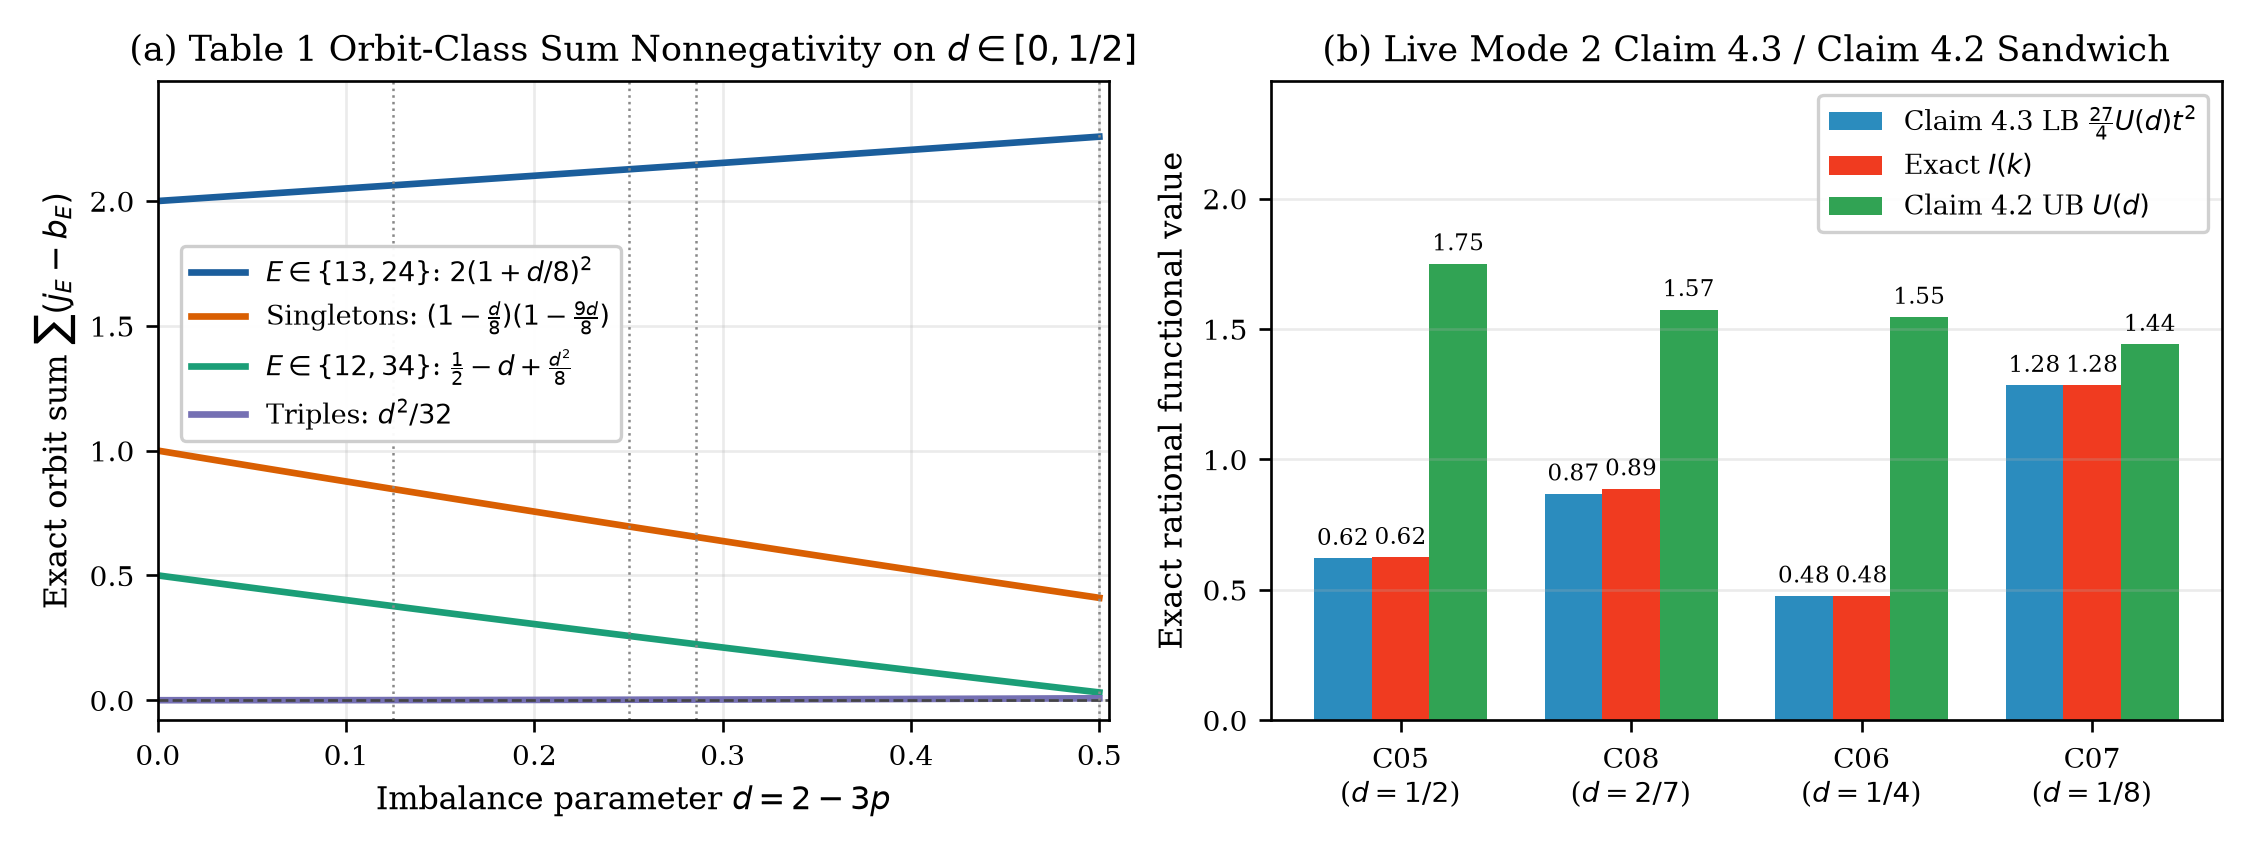
\includegraphics[width=0.90\textwidth]{figures/fig1_table1_sos_profiles.png}
\caption{\textbf{Section~4 SOS Verification.} (a)~Exact rational Table~1 orbit-class sums $\sum (j_E-b_E)$ remain strictly nonnegative over $d=2-3p\in[0,1/2]$. (b)~Live Mode~2 certificates \texttt{C05}--\texttt{C08} satisfy the Claim~4.3--Claim~4.2 sandwich $\tfrac{27}{4}U(d)t^2 \le I(k) \le U(d)$.}
\label{fig:fig1}
\end{figure*}

\paragraph{Worked Witness~1 (Near-Tight Lemma~2.5 and Mode~3a Extremizer, \texttt{C03} \& \texttt{C09}).}
In \texttt{C03}, $n=3$ with $k_{02}=k_{12}=\tfrac{71}{41}$ (a rational convergent below $\sqrt{3}$ since $71^2 = 5041 < 5043 = 3\cdot 41^2$). Every nonzero entry of $C_k$ equals $\tfrac{1}{3}(\tfrac{71}{41})^2 = \tfrac{5041}{5043} < 1$ (for $x,y\in\{0,1\}$ via $k_{x2}k_{y2}$ and for $(2,2)$ via $\tfrac{1}{2}(k_{02}^2+k_{12}^2)$). Hence $\|K\|_2^2 = \tfrac{4}{9}(\tfrac{71}{41})^2 = \tfrac{20164}{15129} \approx 1.33280 \le \tfrac{4}{3}$ ($99.96\%$ of Lemma~2.5's cap) and vertex~2 has row square $\tfrac{10082}{5043} \approx 1.99921 \le 2$. Doubling into $K_{4,2}$ on $n=6$ (\texttt{C09}) yields $t = \tfrac{8}{36}\cdot\tfrac{71}{41} = \tfrac{142}{369}$, giving $27t^2 = \tfrac{20164}{5043} \approx 3.99841 \le 4$ ($99.96\%$ of the Bollob\'as--Gy\H{o}ri limit), with $\mathrm{diag}(A^5)=0$, $w=\tfrac{4}{9}$, and heavy edge $(0,4)$ satisfying $d(0)+d(4)=6 \ge 2wn=\tfrac{16}{3}$.

\paragraph{Worked Witness~2 (Claim~4.3 Sandwich at $d=\tfrac{1}{8}$, \texttt{C07}).}
For $n=8$ with $|X|=5$, $|Y|=3$ ($p=\tfrac{5}{8}, q=\tfrac{3}{8}, d=\tfrac{1}{8}$), setting $k_{xy}=\tfrac{3}{2}$ and $k_{yx}=\tfrac{1}{20}$ yields $t = \tfrac{15}{64}(\tfrac{3}{2}+\tfrac{1}{20}) = \tfrac{93}{256}$, $\beta = \tfrac{3}{256}$, and $C_k \le \tfrac{5763}{6400} < 1$ (on $X^2$; $\tfrac{511}{640}$ on $Y^2$). The Claim~4.2 upper bound is $U(\tfrac{1}{8}) = (2+\tfrac{1}{4})\tfrac{25}{64} + 4\cdot\tfrac{9}{64} = \tfrac{369}{256} \approx 1.4414$, while Claim~4.3 gives $\tfrac{27}{4}U(\tfrac{1}{8})t^2 = \tfrac{86169987}{67108864} \approx 1.2840 \le I(k) = \tfrac{26936133}{20971520} \approx 1.2844 \le \tfrac{369}{256}$, certifying $27t^2 = \tfrac{233523}{65536} \approx 3.5633 \le 4$ (Figs.~\ref{fig:fig1}b and~\ref{fig:fig2}b).

\begin{figure*}[t]
\centering
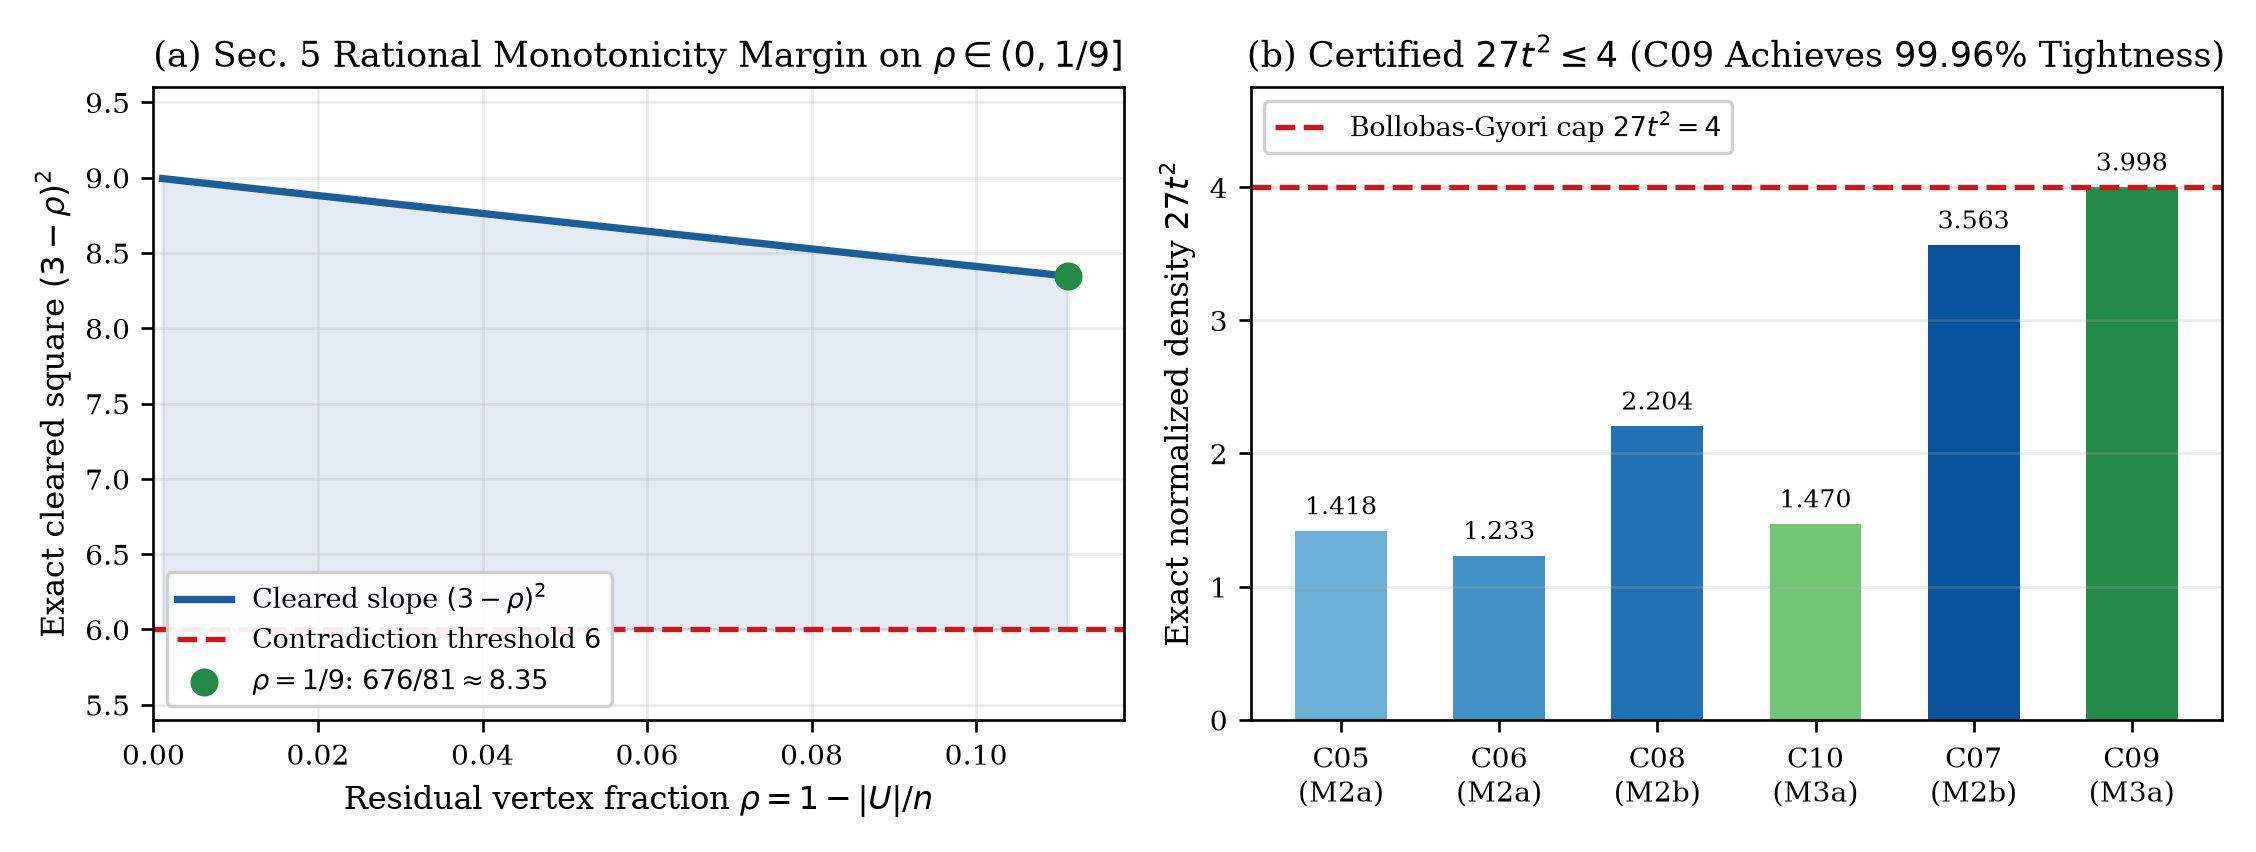
\includegraphics[width=0.90\textwidth]{figures/fig2_rho_monotonicity_and_density.png}
\caption{\textbf{Section~5 Rational Monotonicity and Density Caps.} (a)~Cleared square $(3-\rho)^2$ stays strictly above the threshold $6$ across $(0,1/9]$, reaching minimum $676/81 \approx 8.35$ at $\rho=1/9$ (\texttt{C11}, \texttt{C12}). (b)~Certified $27t^2 \le 4$ across Modes~2--3, with \texttt{C09} reaching $3.9984$.}
\label{fig:fig2}
\end{figure*}

\begin{figure*}[t]
\centering
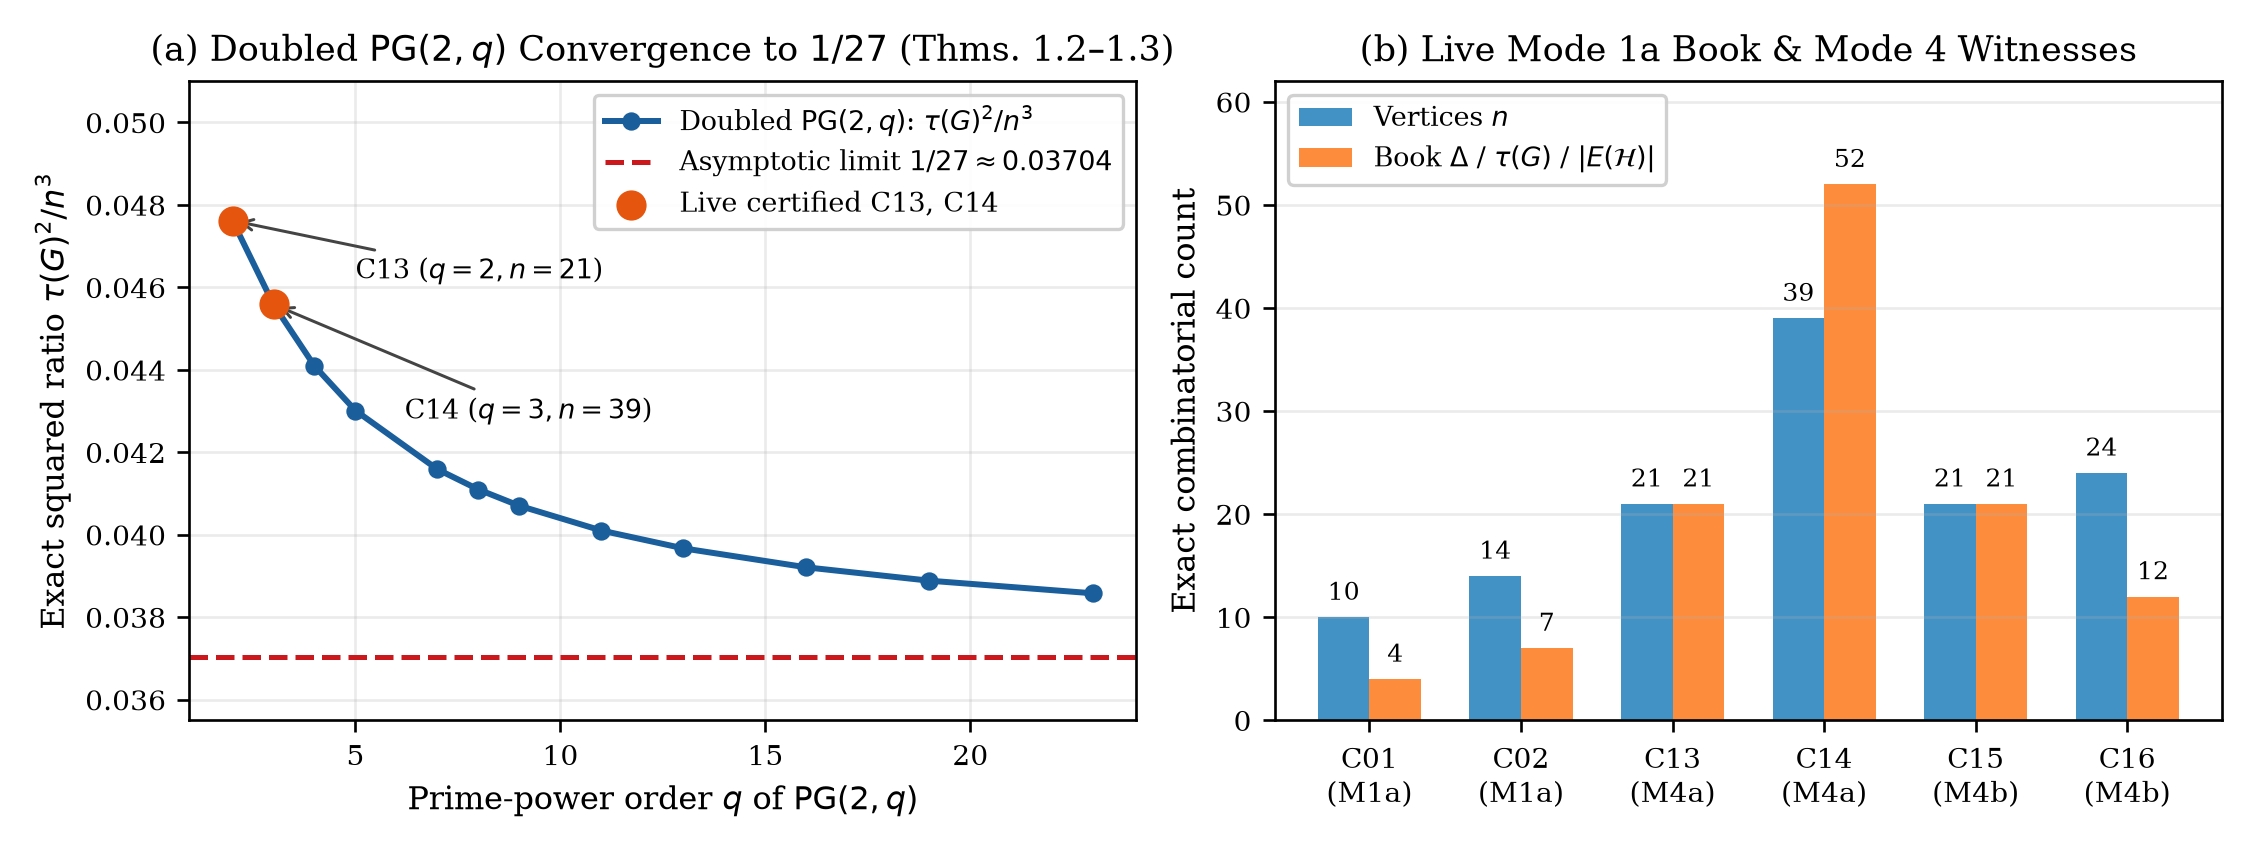
\includegraphics[width=0.90\textwidth]{figures/fig3_bollobas_gyori_and_berge.png}
\caption{\textbf{Extremal Projective-Plane Graphs and Berge 3-Graphs.} (a)~Doubled $\mathrm{PG}(2,q)$ graphs satisfy $\tau(G)^2/n^3 = \tfrac{(q+1)^2}{27(q^2+q+1)} \to \tfrac{1}{27}$ from above (finite-size $+q$ incidence excess), with live certified witnesses \texttt{C13} ($q=2$) and \texttt{C14} ($q=3$). (b)~Exact vertex and structure counts across Mode~1a and Mode~4.}
\label{fig:fig3}
\end{figure*}

\paragraph{Worked Witness~3 (Doubled Projective Planes and Berge 3-Graphs, \texttt{C13}--\texttt{C15}).}
For any prime power $q$, the point-line incidence graph $B_q$ of $\mathrm{PG}(2,q)$ is $C_4$-free with $m_L=m_R=q^2+q+1$ and $|E(B_q)|=(q+1)(q^2+q+1)$. Doubling $L$ produces $G_q$ on $n_G = 3(q^2+q+1)$ vertices with $\tau(G_q)=(q+1)(q^2+q+1)$ triangles and $|E(G_q)|=(2q+3)(q^2+q+1)$ edges. In \texttt{C13} ($q=2$: $n_G=21$, $\tau=21$, $|E|=49$, $\tau^2/n_G^3 = 1/21$) and \texttt{C14} ($q=3$: $n_G=39$, $\tau=52$, $|E|=117$, $\tau^2/n_G^3 = 16/351$), Mode~4a exhaustively verifies both $C_5$-freeness and induced-$C_4$-freeness (Fig.~\ref{fig:fig3}a). Turning the 21 triangles of $G_2$ into a 3-uniform hypergraph (\texttt{C15}) passes Mode~4b's exhaustive DFS check for $\{BC_3, BC_4, BC_5\}$-freeness with $21$ hyperedges and a $C_5$-free 2-shadow, illustrating Theorem~1.4.

\section{Reproducibility and Availability}
All source code, Lean~4 proofs, certificates, figure scripts, and SHA-256 manifest (\texttt{MANIFEST.sha256}) are archived at \nolinkurl{https://github.com/lluiseriksson/triangles-without-pentagons-certificates} under MIT (code/Lean/data) and CC-BY-4.0 (manuscript/figures) licenses. Reproduction requires three commands: \texttt{cd lean \&\& lake build}, \texttt{python -m src.ex\_k3\_c5\_verifier certificates}, and \texttt{pytest -q}.

\paragraph{AI Assistance Disclosure.}
Google Antigravity assisted with Lean~4 proof engineering, zero-float verifier implementation, test/figure automation, and LaTeX drafting. The author verified every mathematical derivation, Lean axiom audit, certificate check, and visual figure inspection, and takes full responsibility for all contents.

\bibliographystyle{plain}
\bibliography{references}
\end{document}
